\documentclass[13pt]{article}
\usepackage[a4paper, total={6.2in, 9in}]{geometry}
\usepackage[utf8]{inputenc}
\usepackage{cmbright}
\usepackage{hyperref} 
\usepackage{graphicx}
\usepackage{amsmath}
\usepackage{amssymb}
\usepackage{parskip}
\usepackage{multicol}
\usepackage{caption}
\usepackage{subcaption}
\usepackage{float}

\title{Flatland Challenge: Report}
\author{Matteo Conti, Manuel Mariani, Davide Sangiorgi}

\newcommand{\figrowtwo}[3]{ %params: subfolder (eg "Policy/Test"), filename1, filename2
    \begin{figure}[H]
        \centering
        \begin{subfigure}[b]{0.49\textwidth}
            \centering
            \includegraphics[width=\textwidth]{assets/Results/#1/#2.png}
        \end{subfigure}
        \hfill
        \begin{subfigure}[b]{0.49\textwidth}
            \centering
            \includegraphics[width=\textwidth]{assets/Results/#1/#3.png}
        \end{subfigure}
    \end{figure}
}

\newcommand{\figrowone}[2]{ %params: subfolder (eg "Policy/Test"), filename1
    \begin{figure}[H]
        \centering
        \begin{subfigure}[b]{0.49\textwidth}
            \centering
            \includegraphics[width=\textwidth]{assets/Results/#1/#2.png}
        \end{subfigure}
    \end{figure}
} 

\begin{document}
\maketitle
\begin{center}
    
    
\includegraphics[width=0.08\textwidth]{assets/unibo.png}\\
    UNIBO \\
    September 2021 \\
    Course: Deep Learning\\
    Professor: Andrea Asperti
    \vspace{2cm}
\end{center}

%
% ============= ABSTRACT ============= 
%
\begin{abstract}
Flatland is a challenge with the objective of efficiently managing dense traffic on complex railway networks. The traffic is composed of trains that are required to go from point A to point B, in the shortest amount of steps and while avoiding collisions. This problem can be solved in multiple ways, from simple controllers to more complex planning algorithms. This project uses \textbf{multi-agent deep reinforcement learning} to solve the problem, alongside with a custom implementation of the environment to aid the task.
\end{abstract}

\begin{center}
    \vspace{2cm}
    
\includegraphics[width=0.4\textwidth]{assets/flatland.png}
\end{center}
\newpage
\tableofcontents
\newpage

%
% ============= INTRODUZIONE ============= 
%

\section{Introduction}
\vspace{0.5cm}

The Flatland's\cite{mohanty2020flatlandrl} objective of handling dense traffic on complex railway networks has gained a lot of interest, so much so that it has been sponsored from the Swiss federal railway and, starting from 2019, AIcrowd has launched a yearly competition in which participants have to find the best solution, evaluated using a standard procedure, for the problem.

The challenge is divided  into two solution categories: Reinforcement Learning and Non-Reinforcement Learning. So far, as of today, Non-RL algorithms have dominated the competition \cite{neurips2020winners}, with the best Non-RL having a score of 297.507/300 points and the best RL solution having a score of 214.15/300 points.

This result is not to be considered a failure of Reinforcement Learning, but rather it should serve to show that RL is a field of Machine Learning and Deep Learning that is still in its early stages, and that there is ample growth margin for novel techniques to be researched. 

This project applies several Deep Reinforcement Learning techniques to this challenging multi-agent environment, such as \textbf{Deep Q Networks} and \textbf{Double Deep Q Networks}, alongside a variety of \textbf{policies} and \textbf{network topologies}, to provide an evaluation of different reinforcement learning methodologies.

In addition, in this project a number of improvements have been implemented to the Flatland environment, such as a \textbf{Binary Tree Observator}, \textbf{Higher level actions} and a physics-inspired \textbf{Reward function}.

%
% ============= FLATLAND ============= 
%

\newpage

%
% ============= FLATLAND ============= 
%

\section{Flatland}
Flatland is a toolkit used to develop and evaluate Multi Agent Reinforcement Learning algorithms\cite{mohanty2020flatlandrl}. The toolkit is used in the Flatland Challenge, an open competition with the main goal of developing an algorithm or a reinforcement learning model to handle a \textit{Vehicle Rescheduling Problem}, in which a number of trains, each with a target railway station, has to navigate a grid of rails, while avoiding collisions and handling malfunctions. 

The objective of the challenge is quite interesting and not trivial: each agent has to both reach its own target in the shortest amount of time while also being cooperative enough to stop itself to give the right of way to incoming trains, and choose another path or wait in case of another agent's malfunction (thus opposing its objective of reaching the target as fast as possible).

\subsection{The Environment}
The Flatland environment is a 2D grid, where each cell corresponds to a possible oriented rail tile (straight, simple switches, crossings and other types of switches) or an empty cell.

\begin{figure}[h]
    \centering
    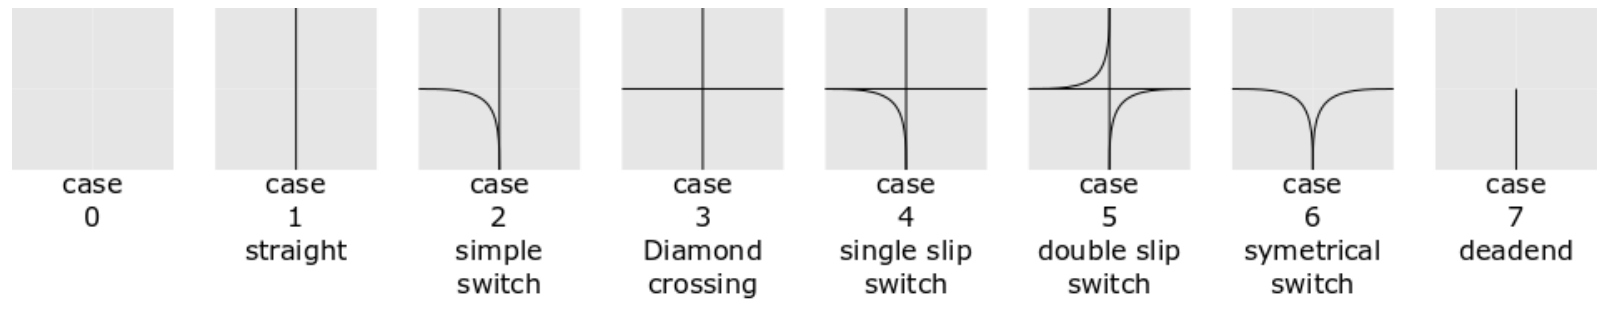
\includegraphics[width=0.8\textwidth]{assets/Flatland/switches.png}
    \caption{Possible railway switches}
    \label{fig:switches}
\end{figure}

When the environment is created, after generating the layout of the railways, a schedule is determined. The schedule assigns to each train a destination (target). When a train reaches its target, by default it is removed from the environment. When all agents are removed, the simulation ends and another episode can start.

\begin{figure}[h]
    \centering
    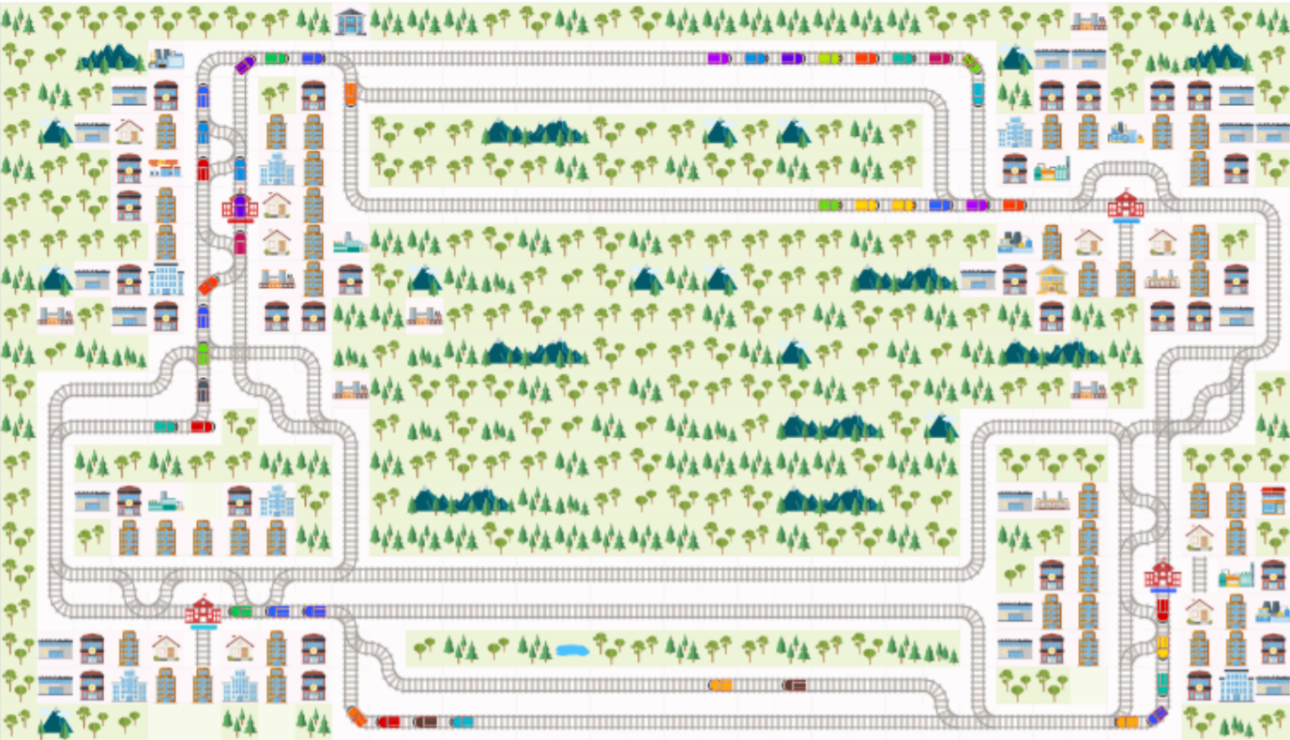
\includegraphics[width=0.8\textwidth]{assets/Flatland/env.png}
    \caption{A Flatland environment}
    \label{fig:env}
\end{figure}

To simulate more realistic conditions, the environment provides the feature to have a different speed rate for each train, and also each train can have a malfunctioning rate, which indicates how often and for how long a train stops abruptly.

\subsection{Action Space}
The possible actions of each agent are limited to the constraints of a railway, meaning it cannot step outside rails and derail, and being a contiguous 2D rail, the agent can only move orthogonally from its current position.

The possible actions are encoded using integers:
\begin{itemize}
    \item \texttt{0} \textbf{Do Nothing}: The agent keeps doing what is doing; if it's moving it keeps moving, if it's stopped it remains stationary.
    \item \texttt{1} \textbf{Deviate Left}: If the agent is at a switch with a transition to its left, the agent chooses that path, otherwise the action has no effect.
    \item \texttt{2} \textbf{Go Forward}: This action starts the agent when stopped and also makes the agent go straight direction at switches.
    \item \texttt{3} \textbf{Deviate Right}: Same as Deviate Left but for right turns.
    \item \texttt{4} \textbf{Stop}: This action stops the agent at its current position.
\end{itemize}

\subsection{Observations}
When the environment is reset or it is advanced to the next timestep, it returns an observation to each agent.

\begin{figure}[h]
    \centering
    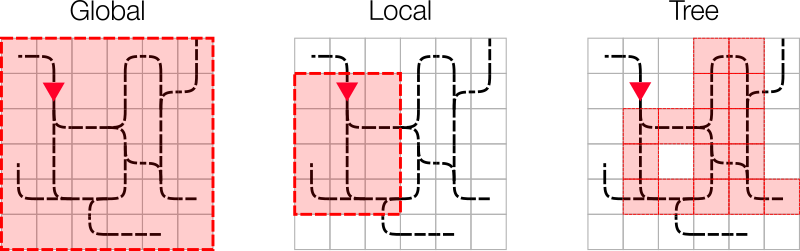
\includegraphics[width=0.6\textwidth]{assets/Flatland/obs.png}
    \caption{A visual summary of the three default Flatland observations}
    \label{fig:fl_obs}
\end{figure}
Flatland provides three default observation types:
\begin{itemize}
    \item \textbf{Global observation}: represents the full flatland environment. It is composed of three channels, with size \texttt{HEIGHT x WIDTH}. The channels are: 
    \begin{itemize}
        \item Transition map: provides an unique value to each type of transition (movement allowed on a cell).
        \item Agent targets: has two sub-channels, one containing the position of the current agent's target and the other has the target for the other agents.
        \item Agent states: Contains 5 sub-channels, representing the position and direction of the agent, position and direction of other agents, trains malfunctions, trains fractional speeds and number of agents ready to depart.
    \end{itemize}
    
    \item \textbf{Local Grid} (deprecated): it is similar to the global observation, but instead of having a global view of the environment the agent has a smaller rectangular view of its surroundings
    
    \item \textbf{Tree Observator}: exploits the fact that a railway network is a graph, and so it build a tree where each node is a rail switch, and its children are the other switches reachable from that point. Each branch is build by looking at the allowed directions (forward, left, backward and right). Missing nodes are assigned a value of \texttt{-inf}. A node cointains 12 channels, and missing values are filled with \texttt{+inf}:
    \begin{itemize}
        \item \texttt{0}: Distance from target, if the target lies on the explored branch.
        \item \texttt{1}: Distance from another agent's target, if detected on the branch.
        \item \texttt{2}: Distance from another agent, if detected.
        \item \texttt{3}: Distance from a possible confict (generated by a predictor), if detected.
        \item \texttt{4}: Distance from an unusable switch
        \item \texttt{5}: Distance to the next node
        \item \texttt{6}: Minimum distance from target if the current path is chosen.
        \item \texttt{7}: Number of agents going in the same direction.
        \item \texttt{8}: Number of agents going in the opposite direction.
        \item \texttt{9}: Malfunctioning / blocking agents fount on the path.
        \item \texttt{10}: Slowest observed speed for an agent in same direction.
        \item \texttt{11}: Number of agents ready to depart
    \end{itemize}
\end{itemize}

\subsection{Rewards and info}
By default, when the state of the environment advances, in addition to the observations, the reward and informations for each agent are returned. A reward can be:
\begin{enumerate}
    \item \texttt{0} if the agent has reached its target
    \item \texttt{-1} otherwise
\end{enumerate}

The informations for each agent include:
\begin{enumerate}
    \item The status of the train (moving, ready to depart, waiting)
    \item Its speed rate
    \item If it's malfunctioning
    \item If an action is required (such as when the environment resets)
\end{enumerate}

\newpage

%
% ============= CUSTOM ENV ============= 
%

\section{Environment Improvements}
In the project, an improved custom version of the Flatland environment has been implemented to aid the training of the agent.

The most substantial improvements have been done in the way observations are presented to the agents, in the actions space and in the reward function.

\subsection{Binarized Tree Observations}
As a baseline the Tree Observator was used. The main limitations of the default implementation are:
\begin{itemize}
    \item \textbf{Missing node values}: in a Tree Observator's Node values are not guaranteed to be present. For example, the \texttt{channel 0}, representing the minimum distance from the target in the current explored branch, more often than not has the value \texttt{+inf} (padding value), since the target won't always lie on the current explored branch (hence its distance is indefinite).
    
    \item \textbf{Empty child nodes}: by default the children of each explored node (switch) are stored in a dictionary, with a key for each of the possible agent's directions. The problem with this is that not all directions are present for a switch. Indeed at every switch, there are always only two possible directions.
    
    \item \textbf{Tree data structure}: in the standard implementation the returned observation is a tree, where, starting from the Root node, each node points to its children using references. Since in the project Neural Networks are used, which generally take in input array or tensors, using such data structure is unfeasible.
\end{itemize}

To address these issues, a custom implementation of the Tree Observer has been done.

\subsubsection{Nodes}
Missing values by default are set to a \texttt{+inf} value. Generally neural networks do not accept those values. To fix this issue, \texttt{+inf} padding values have been remapped to be of arbitrary high constant size.

Also, to limit the size of the observation space, the values are normalized to $[-1, 1]$ by dividing the values with the previously defined padding constant.

In addition, the Node has been augmented with more values:
\begin{itemize}
    \item Train current position.
    \item Left and Right children, which purpose will be explained thoroughly in the next section .
    \item Target is on explored branch flag.
    \item Number of unusable switch in the explored branch. An unusable switch is a switch that cannot be used in the current direction, but can if the train were directed in the opposite way, (for example the simple switch shown in case 2 of figure \ref{fig:switches} is counted as unusable if the train had a south direction).
\end{itemize}

\subsubsection{Tree vectorization and binarization}
To binarize the tree, instead of having a branch for each direction (left, forward, right, backward), the branches are associated to a "generic" direction, meaning the first and second possible choices.

After the missing branches are pruned, each node is vectorized (meaning its numerical informations are stored in a simple vector). Finally, with all the node contents vectorized, the tree is explored using a \textit{breadth first} search and the explored contents are procedurally put into a final array.

\subsection{Actions}
The environment has also been modified to support the binary tree observator and to allow better multi-agent training.

\subsubsection{Higher Level Actions}
Since the observation is a binary tree, the actions also get remapped into a binary choice, in terms of direction, plus another choice for the stop action. So in total we have three "high-level" actions:
\begin{itemize}
    \item \texttt{0}: Leftmost choice
    \item \texttt{1}: Stop
    \item \texttt{2}: Rightmost choice
\end{itemize}

The high-level actions, before being passed to the original Flatland method to advance the simulation, are then reconverted into Flatlands "low-level" actions (\texttt{0,..., 4}) by looking at the allowed transitions, considering also the train's direction, that the agent can go and choosing the corresponding low-level action.

For example, with a simple switch oriented to the right (see case 2 of figure \ref{fig:switches}), and a train going north, the high level actions will get converted into:
\begin{itemize}
    \item[] \texttt{0} Leftmost $\to$ \texttt{1} Left
    \item[] \texttt{1} Stop $\to$ \texttt{4} Stop
    \item[] \texttt{2} Rightmost $\to$ \texttt{2} Forward
\end{itemize}
In the dual case of a right oriented simple switch, the leftmost action would be remapped to going forward, and the rightmost into going right.

\subsubsection{Required actions}
By default the Flatland environment expects all actions of the trains for each step. On straightaways though, the train action is not required, since the only actions a train can do is keep going forward or stopping. When in a straight rail, if an action such as "left" or "right" would keep the train going forward, despite the correct action being "forward". Also, stopping in the middle of a straightaway wouldn't have much sense.

Hence, to aid the agent's  training, on straightaways the choice of going forward is enforced: the action is fixed to \texttt{2} (go forward) and the observation-action-reward tuple is not stored in the agent's learning memory.

Only before and in the middle of switches the agent's action is required, which is checked by counting the number of allowed directions in correspondance with the agent's position.

\subsection{Reward Function}
The Flatland default reward function is, for each agent, \texttt{-1} if the agent has not reached the target, \texttt{0} otherwise.

To aid the agent's training, we implemented a physics-based reward function, that gives higher rewards when the agent gets closer to its target, and also gets lower when an agent is facing another agent in a straightaway. The first part of the function encourages the agent to go as close as possible to the target, while the second part discourages the agent into running across trains that are facing the opposite direction (to avoid crashes and deadlocks).

The function uses two parameters:
\begin{itemize}
    \item[] Target Mass, $m_T$
    \item[] Agent Mass, $m_A$
\end{itemize}

Then at each environment step $k$, for each agent $i$ the reward is calculated as follows:
\begin{enumerate}
    \item Consider the Manhattan distance from the agent's position to its target: $d_{T}(i, k)$
    \item Set the reward (positive) to the target gravitational:
    \begin{equation*}
        r_i(k) = \begin{cases}
            \frac{m_T}{{d_{T}(i, k)}^2} \quad \text{if} \quad d_{T}(i, k) \neq 0 \\
            2 \ m_{T} \quad otherwise
        \end{cases}
    \end{equation*}
    \item Then calculate the gravitational force $g_{i,j}(k)$ for each other agent $j$ by looking at the "railway distance" $d_{T}(i, k)$ (the distance in number of explored railway tiles found by the observator), considering only agents that are in the opposite direction of the agent $i$:
    \begin{equation*}
        g_{i,j}(k) = \begin{cases}
        0 \quad \text{if direction $i$ not opposite direction $j$} \\
        \frac{m_A}{{d_{T}(i, k)}^2} \quad \text{if} \quad d_{T}(i, k) \neq 0 \\
        100 \ m_A \quad \text{if} \quad d_{T}(i, k) = 0
        \end{cases}
    \end{equation*}
    \item And finally subtract all the agents' gravitational forces from the reward:
    \[r_i(k) = r_i(k) - \sum_{j, \ j\neq i} g_{i,j}(k)\]
\end{enumerate}

%
% ============= REINFORCEMENT LEARNING ============= 
%

\newpage

%
% ============= RL ============= 
%

\section{Reinforcement Learning}
To solve a task such as the Flatland Challenge, in which there is an agent or more, interacting with an environment, there exist numerous techniques. Some of the most classical ones include: planning algorithms\cite{goosuerw2004models}, optimization techniques\cite{nedic2009distributed}, explicit control algorithms and PID loops\cite{yuan2018uncoupled}.

Those techniques require an extensive knowledge about the problem's domain (for algorithms), or extensive parameter tuning (control algorithms and PID loops).

In recent years, a novel group of deep learning techniques, inspired by cognitive-neuroscience, has been developed: \textbf{Reinforcement Learning}\cite{kaelbling1996reinforcement}.

In nature, any \textit{agent} (animal) lives in an \textit{environment} which responds to the agent's \textit{action}, and the agent can gain \textit{benefit} or detriment (reward) based on the outcome of its action, both in the immediate and in the long term.

By a combination of instinctual and a learnt knowledge about the environment, the agent is capable of choosing the action which is more beneficial to it, while trying to avoid harmful action. The process of learning which actions are better and which are worse is at the core of reinforcement learning.

This notion has been modeled using two main entities:
\begin{enumerate}
    \item \textbf{Environment}: 
        a dynamic and observable system, capable of receiving inputs (actions) that affect its state and providing feedback (rewards) to the entity that provided the input.
    \item \textbf{Agent}: 
        an entity capable of observing the environment, deciding what is the best action given the current observation through a \textbf{policy} and capable of improving its policy through a \textbf{reinforcement learning algorithm} which takes into account the reward given by the environment
    
\end{enumerate}
\begin{figure}[h]
    \centering
    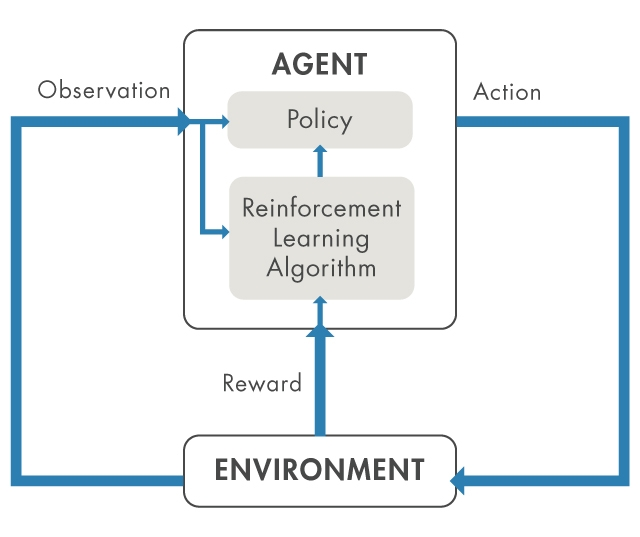
\includegraphics[width=0.4\textwidth]{assets/Reinforcement Learning/rl.png}
    \caption{Reinforcement learning actor-environment loop}
    \label{fig:_label}
\end{figure}

\subsection{Reinforcement Learning Algorithms}
\subsubsection{Q-Learning}
The simplest and one of the first reinforcement learning algorithms is called \textbf{Q-Learning}\cite{watkins1992q}. The basis of the algorithm is a table $Q$ that maps state-action pairs into numeric values, called Q-values representing the "quality" of a particular action in a given state.
\[Q: S \times A \to \mathbb{R} \]
Since the environment is a dynamic system which evolves over the course of the action sequence, so do the rewards. For example, an action might not give an immediate reward when it is performed, but only at the end of the sequence of action. So the Q-learning algorithm also takes into account the \textbf{temporal difference} when updating its value in the learning process:
\[Q^{new}(s_t, a_t) \leftarrow Q(s_t, a_t) + \alpha \cdot [r_t + \gamma \cdot \max_a{ Q(s_{t+1}, a_t)} - Q(s_t, a_t)] \]
where $s_t, a_t, r_t$ are the state, action and reward in the timestep $t$; $alpha$ is the \textit{learning rate}, which determines the effect new information has on the learning process compared to the old one, and $\gamma$ is the \textit{discount factor}, which weights the maximal expected reward of the state in the next timestep.

\subsubsection{Deep Q-Learning}
As the dimension of the state and action spaces increase, for example in environments with continuous multi-dimensional state or action spaces, 
the size of the Q-table increases combinatorially. To overcome this issue in \textbf{Deep Q-Learning}\cite{mnih2013playing}, instead of relying on discrete tables, a neural network is used to approximate the Q-values.

Instead of mapping state-action pairs to a single Q-value, a Deep Q-Network maps a state to $n$ Q-values, where $n$ is the number of possible agent's actions.

\begin{figure}[h]
    \centering
    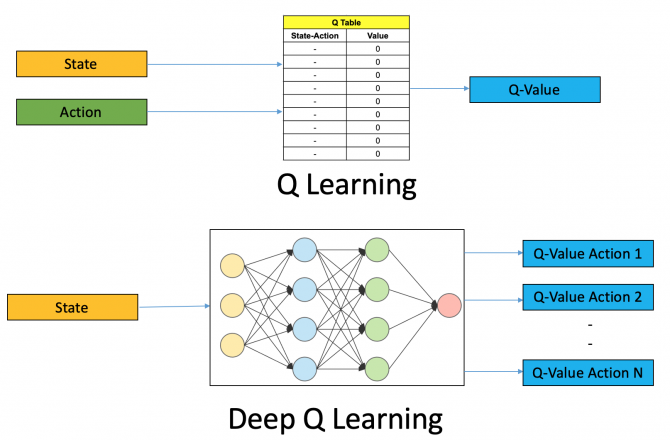
\includegraphics[width=0.4\textwidth]{assets/Reinforcement Learning/q-vs-dqn.png}
    \caption{Q-Learning and Deep Q-Learning compared}
    \label{fig:q-vs-dqn}
\end{figure}

The loss function used in the neural network training is the distance from the expected value of the Q-table and the prediction, using the following Bellman's equation:
\[L(\theta) = (\mathbb{E}_{s'}[r + \gamma \max_{a'}{Q(s',a')]} - Q(s,a,\theta))^2 \]

To compute the loss, a tuple containing $(s_i, a_i, r_i, s_{i+1})$ is stored into an experience memory, and it is replayed during training using a random or prioritized sampling.

\subsubsection{Double Deep Q-Learning}
Using a simpler DQN there is a constant overestimation bias of Q-values due to the fact that we are updating both the approximated target $[r + \gamma \max_{a'}{Q(s',a')}]$ and the current estimation $[Q(s,a,\theta)]$. To solve this, \textbf{Double Deep Q-Learning}\cite{van2016deep} uses a two networks with parameters $\theta$ and $\theta'$, instead of one, each of which is used to update the other during training using the following loss function:
\[L(\theta) = (\mathbb{E}_{s'}[r + \gamma Q(s', \overline{a} | \theta')] - Q(s', a' |\theta))^2\]
\[\overline{a} = \arg\max_{a'}{Q(s',a' | \theta)}\]

Then during training the two networks alternate their role periodically, thus providing a better unbiased estimate for the Q-value of the action.

\subsection{Policies}
A policy is a function $\pi(a | s)$ is a function that, given an action $a$ in a state $s$, returns the probability of the agent choosing the action $a$.

Usually in deterministic environments, the agent will always choose the action that grants it the best possible reward. This policy is known as a \textbf{Greedy Policy}.

In a training environment, however, we cannot apply a Greedy Policy. Since at the beginning of the training the agent does not know what's the best action to take, with a greedy policy the same sub-optimal action $\overline{a}$ would be repeated for each state $\overline{s}$, thus the agent would not be capable of exploring new actions (with better or worse rewards) for that particular state, leading the learning process into a local maxima.

On the other hand, if the agent were to take actions at random, the agent would explore many possible actions but would not actually learn the optimal policy, thus a compromise between exploration and exploitation is needed.

\subsubsection{Epsilon Greedy Policy}
The Epsilon Greedy Policy chooses between the exploitation of the best learnt action and the exploration of new actions randomly. To do so, a random number $r$ is generated and if it's value is less than the $\epsilon$ parameter, a random action is explored, otherwise the current best action is exploited.

\subsubsection{Softmax Policy}
The Softmax Policy 
%{\cite{mei2020global}} 
chooses an action based on the output of the Q-Network. It uses the softmax function to obtain the actions' probabilities distribution, which is then used to determine randomly the chosen action. This means that actions with higher values are more likely to get chosen, but there it is still exploration due to the aleatory nature of the process.

\subsubsection{Boltzmann Policy}
Like the Softmax Policy, the Boltzmann Policy uses a softmax function to determine the actions' probability distribution. The main difference is that the softmax function used has a parameter called \textit{temperature} $\tau$ used to control the spread of probabilities across actions.
\[ P(a_i) = \frac{e^{Q(a_i) / \tau}}{\sum_a e^{Q(a)/\tau}}\]

Higher temperatures cause the actions to be all nearly equiprobable, while lower temperatures increase the difference in selection probabilities for actions that that differ in their value. For $\tau \to 0$, the policy behaves in the same manner as a Greedy Policy.

\subsubsection{Linear Annealing Policy}
The Linear Annealing Policy is a meta-policy which affects the parameter used by an internal policy over the course of the training. For example it can be used with the Boltzmann Policy to decrease the temperature $\tau$ over the course of the training, resulting in more exploitation end less exploration as the training progresses.

The parameter affected by this policy starts at a certain value and it reaches an end value using a linear function of the number of episodes. Other variations exist, that instead of a linear function use a quadratic, exponential, sinusoidal or other types of functions.
\newpage
%
% ============= NEURAL NETWORKS ============= 
%

\section{Neural Networks}
In the project, a selection of neural network architectures have been implemented, to test their performance relatively to speed of training (convergence) and also their capabilities of solving the Flatland Challenge in the evaluation phase.

All networks used are simple \textbf{Sequential} networks (Feed Forward), and the main differences lie in their topology or number of parameters.

All three networks share the same inputs and outputs:
\begin{enumerate}
    \item \textbf{Input}: the input is provided by the Binary Tree Observator as an array of size \texttt{N EXPLORED NODES} $\times$ \texttt{N FEATURES PER NODE}. The number of explored nodes is 15 (given by a tree exploration depth of 4) and the number of parameters is 16, thus the input node has size 240.
    \item \textbf{Output}: since we are using Q-Learning Algorithms, the output layer of the networks must encode the Q-Values of each actions. Therefore by using the previously defined "Higher Level Actions", we only have 3 possible actions (instead of the default 5), resulting in an output layer of size 3.
\end{enumerate}

\subsection{Sequential 1}
\begin{center}
    \begin{tabular}{| l | c | r |}
        \hline
        \multicolumn{3}{|c|}{\textbf{Sequential 1 Architecture}} \\
        \hline
        \hline
        \textbf{Layer and Type} & \textbf{Output Shape} & \textbf{No. Parameters} \\
        \hline
        Flatten input & 240 & 0 \\
        Dense 1 & 512 & 123,392 \\
        Dense 2 & 256 & 131,328 \\
        Dense 3 & 128 & 32,896 \\
        Dense output & 3 & 387 \\
        \hline
        \multicolumn{2}{|l|}{\textbf{Total parameters:}} & 288,003 \\
        \multicolumn{2}{|l|}{Trainable parameters:} & 288,003 \\
        \multicolumn{2}{|l|}{Non trainable parameters:} & 0 \\
        \hline
    \end{tabular}
\end{center}

The first neural network implemented, named "Sequential 1", is a sequence of 4 \textit{Biased} Dense layers, where the first three are activated using the \textbf{ReLU} function, and the last layer uses a \textbf{Linear} activation function.

The objective of this network is to provide a baseline for comparison, with its main characteristic of having a relatively \textit{high amount of parameters}.

\subsection{Sequential 2}

\begin{center}
    \begin{tabular}{| l | c | r |}
        \hline
        \multicolumn{3}{|c|}{\textbf{Sequential 2 Architecture}} \\
        \hline
        \hline
        \textbf{Layer and Type} & \textbf{Output Shape} & \textbf{No. Parameters} \\
        \hline
        Flatten input & 240 & 0 \\
        Dense 1 & 256 & 61,696 \\
        Dense 2 & 128 & 32,896 \\
        Dense 3 & 256 & 33,024 \\
        Dense output & 3 & 771 \\
        \hline
        \multicolumn{2}{|l|}{\textbf{Total parameters:}} & 128,387 \\
        \multicolumn{2}{|l|}{Trainable parameters:} & 128,387 \\
        \multicolumn{2}{|l|}{Non trainable parameters:} & 0 \\
        \hline
    \end{tabular}
\end{center}

The "Dense 2" network shares the same architecture with the "Sequential 1", with the main difference of having a \textit{modestly reduced amount of parameters} in its Dense layers.


\subsection{1D Convolutional}
\begin{center}
    \begin{tabular}{| l | c | r |}
        \hline
        \multicolumn{3}{|c|}{\textbf{1D Convolutional Architecture}} \\
        \hline
        \hline
        \textbf{Layer and Type} & \textbf{Output Shape} & \textbf{No. Parameters} \\
        \hline
        Flatten input & 240 & 0 \\
        Reshape & (15, 16) & 0 \\
        Conv1D 1 & (15, 16) & 272 \\
        Conv1D 2 & (15, 16) & 272 \\
        Conv1D 3 & (15, 8) & 136 \\
        Conv1D 4 & (15, 4) & 36 \\
        Flatten & 60 & 0 \\
        Dense 1 & 64 & 3,904 \\
        Dense 2 & 32 & 2,080 \\
        Dense 3 & 16 & 528 \\
        Dense 4 & 16 & 272 \\
        Dense output & 3 & 51 \\
        \hline
        \multicolumn{2}{|l|}{\textbf{Total parameters:}} & 7,551 \\
        \multicolumn{2}{|l|}{Trainable parameters:} & 7,551 \\
        \multicolumn{2}{|l|}{Non trainable parameters:} & 0 \\
        \hline
    \end{tabular}
\end{center}

The main concept of this network, named "1D Convolutional", is to apply a \textbf{dimensionality reduction} to the inputs, and then use the reduced inputs into a \textbf{Main-Q-Network} to determine the Q-Values.

Conceptually, the networks works as follows:
\begin{enumerate}
    \item The one dimensional output is reshaped into a matrix of shape \texttt{(N EXPLORED NODES, N FEATURES PER NODE)}.
    \item Then the matrix is pre-processed using a series of 1D convolutional layers that gradually reduce the dimension of the input matrix; this reduction can also be empirically thought as the pre-processor assigning a "quality value vector" to each node.
    \item The output matrix of the pre-processor is then flattened into a 1D array
    \item Finally, the array containing the pre-processed node values is then used by the Main-Q-Network to select the best possible node (hence the best possible action), returning the actions' Q-Values
\end{enumerate}

The sequence of Conv1D layers, which is referred as the "Pre-processor", uses 1D Convolutional Biased layers with kernel size set to 1, to process each node \textit{individually}, no padding (due to the kernel size being 1), and a variable amount of output nodes. Performing one dimensional convolution such as those is akin to applying the same sequence of dense layers along a direction of the matrix, thus we can think of the pre-processor as a "sub-network" being applied to each node.

The main feature of this architecture is the \textit{greatly reduced amount of parameters}, due to the facts that each of the 15 nodes gets pre-processed using a sub-network with the same parameters (716) and then the input of the Main-Q-Network receives just 60 inputs (compared to the previous 240), reducing the need of a higher number of parameters (6835).

Also the overall number of trainable parameters in the Main-Q-Network has been chosen to be very low, approximately $\frac{1}{40}$ of the "Dense 1" and $\frac{1}{20}$ of the "Dense 2", to experiment with the effects of a very low number of parameters on training convergence speed and the network's generalization capabilities.


\newpage

%
% ============= RESULTS ============= 
%

\section{Results}
The following section shows a series of experiments comparing the benefits of the networks and algorithm concepts presented so far.

The experiments are a series of independent tests on the performance, both in training and evaluation, of four key concepts, each answering a claim:
\begin{itemize}
    \item \textbf{Network Architecture}. Which architecture converges more quickly? Which one performs the best in tests?
    \item \textbf{Policy}. Which is the policy that improves the learning-phase the most?
    \item \textbf{Number of agents}. What is the effect of the number of agents on the general performances, using the best network and policy?
    \item \textbf{Reinforcement Learning algorithm}. Which RL algorithm grants more improvements?
\end{itemize}

% % %

\subsection*{Plots Guide}
Most of the plots have been generated using WANDB. In the plot legends, the name of the run is shown, formatted as follows:
\begin{center}
    \texttt{(train / test) <RL-Algorithm>-<Policy>-<Network Type>-<No.Agents>}
\end{center}

The WANDB plots' titles represent:
\begin{itemize}
    \item \texttt{reward\_mean}: the mean reward of all agents per step, for each episodes.
    \item \texttt{target\_reached\_in\_steps}: the amount of steps that all agents have taken to reach their target, normalized by the number of agents. If an agent has not reached the target by the end of the allowed number of steps (500 max steps), the maximum value is assigned.
    \item \texttt{action\_mean}: since all values have a numeric value associated with them (0, 1, 2), the mean of all performed actions can be calculated to get a grasp on what are the agent's preferred actions.
    \item \texttt{\% Actors completed}: in multi-actor training, it represents the percentage of actors that have managed to reach their target in steps less than the maximum threshold.
\end{itemize}

On the x-axis the number of episodes in the run is displayed, which is 100 for testing, and slightly variable for training episodes. This variance is due to the fact that training is guaranteed performed for a minimum number of episodes(1000), but it's stopped only when the cumulative number of steps taken during all the episodes exceeds a threshold (500000).

All values displayed in the y-axis are smoothed using a running average with window of 50 for training plots, and of 20 for testing.

% % %

\subsection{Network Architectures}
In this section, we try to compare the performances of different network architectures both in the train and in the evaluation flows.

To obtain meaningful results, we have train/tested our environment leaving unchanged all of the others configurations. 
In particular, we have used an Epsilon Greedy policy, a DQN algorithm and a fixed number of agents equal to 1.

\subsubsection*{Training}
We tested the performance of the chosen policies considering mainly two parameters of our trainings: the reward mean and the number of steps needed to reach the target.

\figrowtwo{Architecture/Train}{reward_mean}{target_reached_in_steps}
Looking at the \emph{target\_reached\_in\_steps} plot, we can see that, despite the relevant differences in the first 250 episodes, the networks seem to produce an equal average of steps necessary to reach the target. \\
In general, we can also observe that the "sequential-2" network has a better average behaviour during all the training.\\

The \emph{reward\_mean} plot mainly confirms the behaviour described above.

\subsubsection*{Evaluation}
\figrowtwo{Architecture/Test}{reward_mean}{target_reached_in_steps}
\figrowone{Architecture/Test}{action_mean}

Looking at the \emph{target\_reached\_in\_steps} plot, we can mainly see three different behaviours. 

The first one is that of "sequential-1" network which is the worst because it produces an averaged result that, in summary, means "agents never arrives".
The second one is that of "conv-1" which produces an average result where the majority of the agents don't arrive at the target.
The third one is that of "sequential-2" network, which is, as expected, the better.

Indeed, by looking at the \emph{action\_mean} plot we can observe that the "sequential-1" network (which is the worst one) mainly choose the STOP action, while the "sequential-2" mainly choose the LEFT-ORIENTED action and the "conv-1" mainly choose the RIGHT-ORIENTED action.
This reflects the three different behaviors of the networks.

Overall, the fact that "sequential-2" performed the best suggests that a middle ground of number of parameters is the most appropriate choice; "sequential-1", having 288,003 parameters, doesn't learn quickly enough to perform adequately in evaluation, while the "conv-1" network, with lot less parameters (7,551) performs better than the "sequential-1". Further work is needed to prove if, with an higher number of parameters and more training time, the "conv-1" is an adequate network for the challenge.

% % %

\subsection{Policies}
We wanted to test two different policies, the Epsilon Greedy policy and the Boltzman policy. To compare the result we fixed the number of agents equal to 1 and selected always the same network, the “Sequential 1” previously described.

\subsubsection*{Training performance}

We tested the performance of the chosen policies considering mainly two parameters of our trainings: the reward mean and the number of steps needed to reach the target.

\figrowtwo{Policy/Train}{reward_mean}{target_reached_in_steps}

The reward mean reveals only local differences and not an evident change in the results, but considering only one policy at a time we can observe two slightly different trends. The Boltzmann policy presents two main peaks but not a global increment, while we can notice an improvement in performances in case of Epsilon Greedy policy. 

The analysis of the second graph can be divided into three intervals: from episode 0 to $\approx$250, from episode $\approx$250 to $\approx$1500 and from episode $\approx$250 to the end.

In the first interval we can observe a similar behaviour, but then the Boltzmann policy seems to perform better than the Epsilon Greedy. In the final steps however Boltzmann has a peak in the number of steps needed to reach the target, while the negative slope of the Epsilon Greedy is coherent with previous oscillations.

In this case we do not have a comparison between train and test because, as explained before, in the test only the Greedy policy was adopted.

% % %

\subsection{Number of agents}
In this section we compare the effects the number of agent has on both training and evalutation performance, using the best performing network and policy configurations.

The runs are of 1, 2 and 3 agents. These numbers were chosen because, due to how the map was generated and the simulations ran, higher number of agents are not feasible. In particular, the map size was not chose particularly big to speed up the training process and, because of this, with higher number of agents, crashes between trains would happen too frequently to usefully train the network, in conjunction with the fact that when two trains collide, the simulation is reset.


\subsubsection*{Training performance}
\figrowtwo{Agents/Train}{reward_mean}{target_reached_in_steps}

As expected, the training performance is worse for environments with 3 agents. On the other hand, with 2 agents the performance is not too different from the single agent environment. Considering also the fact that the number of training episodes is the same for all three simulations, a more proportionate estimation of the performance is appropriate, with longer training periods for environments with more agents.

\subsubsection*{Evaluation}
\figrowtwo{Agents/Test}{reward_mean}{target_reached_in_steps}
\figrowtwo{Agents/Test}{action_mean}{perc_agents_completed}

In line with the training performance observations, the percentage of agent reaching the target in useful time is considerably smaller for the 3 agents environment; while the performance of the environment with 2 agents is comparable to the one with 1 agent considering also the same training steps.

% % %

\subsection{DRL Algorithms}
Keeping fixed the “Sequential 2” network and the Boltzman policy, we applied different deep reinforcement learning algorithms: the deep q network, the double deep q network and the dueling double deep q network. We chose to compare the results on the environment with two agents.

\subsubsection*{Training performance}
\figrowtwo{RLAlgorithms/Train}{reward_mean}{target_reached_in_steps}

Surprisingly, the training plots show that the DQN has much better performance compared to the DDQN.

In particular, the \emph{target\_reached\_in\_steps} plot shows that the DQN reaches the target in a much lower amount of steps, while the Double has values of around the maximum, suggesting sub-par learning performance.

\subsubsection*{Evaluation}
\figrowtwo{RLAlgorithms/Test}{reward_mean}{target_reached_in_steps}
\figrowtwo{RLAlgorithms/Test}{action_mean}{perc_agents_completed}

Coherently to the previous results, the DDQN saturates the number of steps needed to reach the target and, as consequence, the corresponding reward is minimum, while the DQN performs highly better. In particular the target is reached by the DQN in a limited amout of steps.Coherently to the previous results, the DDQN saturates the number of steps needed to reach the target and, as consequence, the corresponding reward is minimum, while the DQN performs highly better. In particular the target is reached by the DQN in a limited amount of steps.

\newpage

%
% ============= CONCLUSIONS ============= 
%

\section{Final remarks}

\vspace{0.5cm}

This project has proved itself to be quite challenging but an excellent way to learn first-hand how to design and develop Reinforcement Learning algorithms to tackle complex environments. \\
\newline

Developing the \textbf{improvements in the environment} has been an interesting chance to think in a creative way and to put in practice algorithm design principles.\\ 
The implementation of \textbf{Reinforcement Learning Algorithms} and \textbf{Neural Networks} was a great way to learn RL concepts, alongside improving the required soft-skills of reading research papers and, just as important, libraries' documentation and source code understanding of libraries such as Tensorflow, Keras, Keras-RL and WANDB. \\
\newline

Finally, we learnt to have patience, and that Reinforcement Learning is a trial-and-error process that requires a general understanding of both the environment and of how the algorithm works, but most importantly we learnt that intuition is an invaluable skill in this kind of tasks.

Overall, even if our solution didn't reach state-of-the-art quality, we are very satisfied of our accomplishments, because we learnt many useful skills that will endure throughout our academic and working life.

\newpage

%
% ============= BILBIOGRAPHY ============= 
%

\bibliographystyle{unsrt}
\bibliography{biblio}
\end{document}

